\section{Objective}\label{obj}

The aim of this project is to estimate the distance between the camera and the object. Only the intrinsic matrix shall be used to estimate the distance. However, since the distance cannot be calculated with the intrinsic matrix alone the following further conditions are assumed:

\begin{itemize}
    \item We assume the checkerboard to be perpendicular to the camera.
    \item The full size of the checkerboard is exactly 50 cm by 50 cm.
\end{itemize}

With this additional information, we can infer the possible distance based on the pixel spacing in the image. To achieve this recordings have been provided as a source. In these, a 8x8 checkerboard is placed by a person in different positions and at different angles to the camera. These frames in the recordings are the basis for the camera calibration, which is to be carried out per recording.\\

In figure \ref{fig:schwalbe_og} and figure \ref{fig:printer_og} one can see the objects for which the distance is to be estimated.
\begin{figure}[H]
     \centering
     \captionsetup{justification=centering}
     \begin{minipage}[b]{0.5\textwidth}
        \centering
        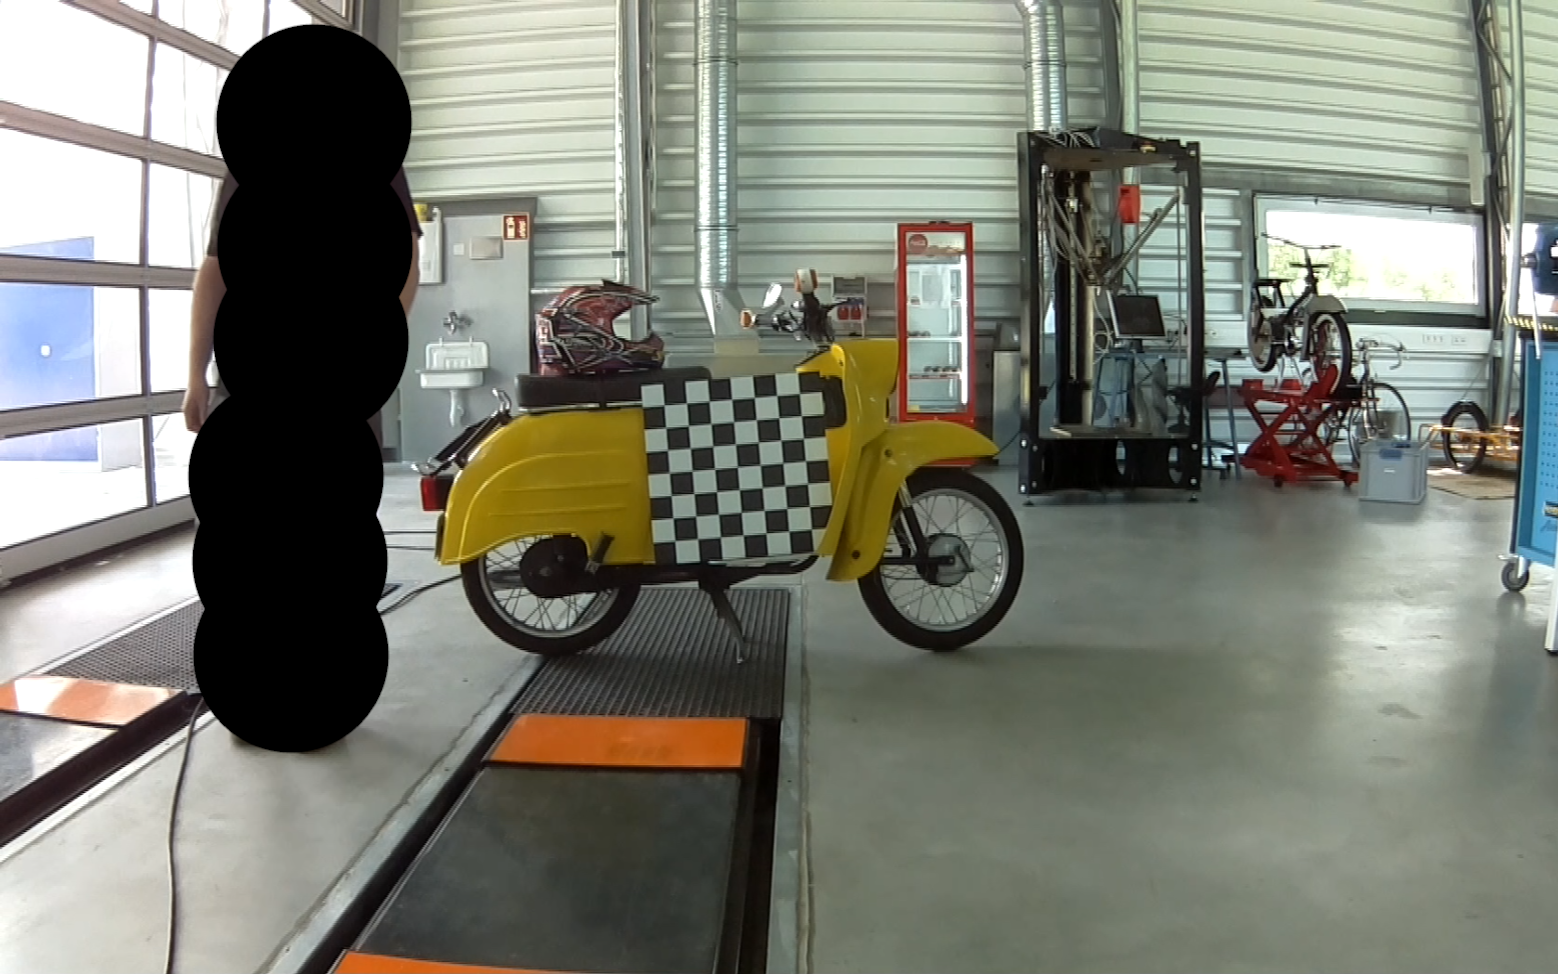
\includegraphics[width=.95\textwidth]{image/1/schwalbe.png}
        \caption{Object Schwalbe}
        \label{fig:schwalbe_og}
     \end{minipage}%
     \begin{minipage}[b]{0.5\textwidth}
        \centering
        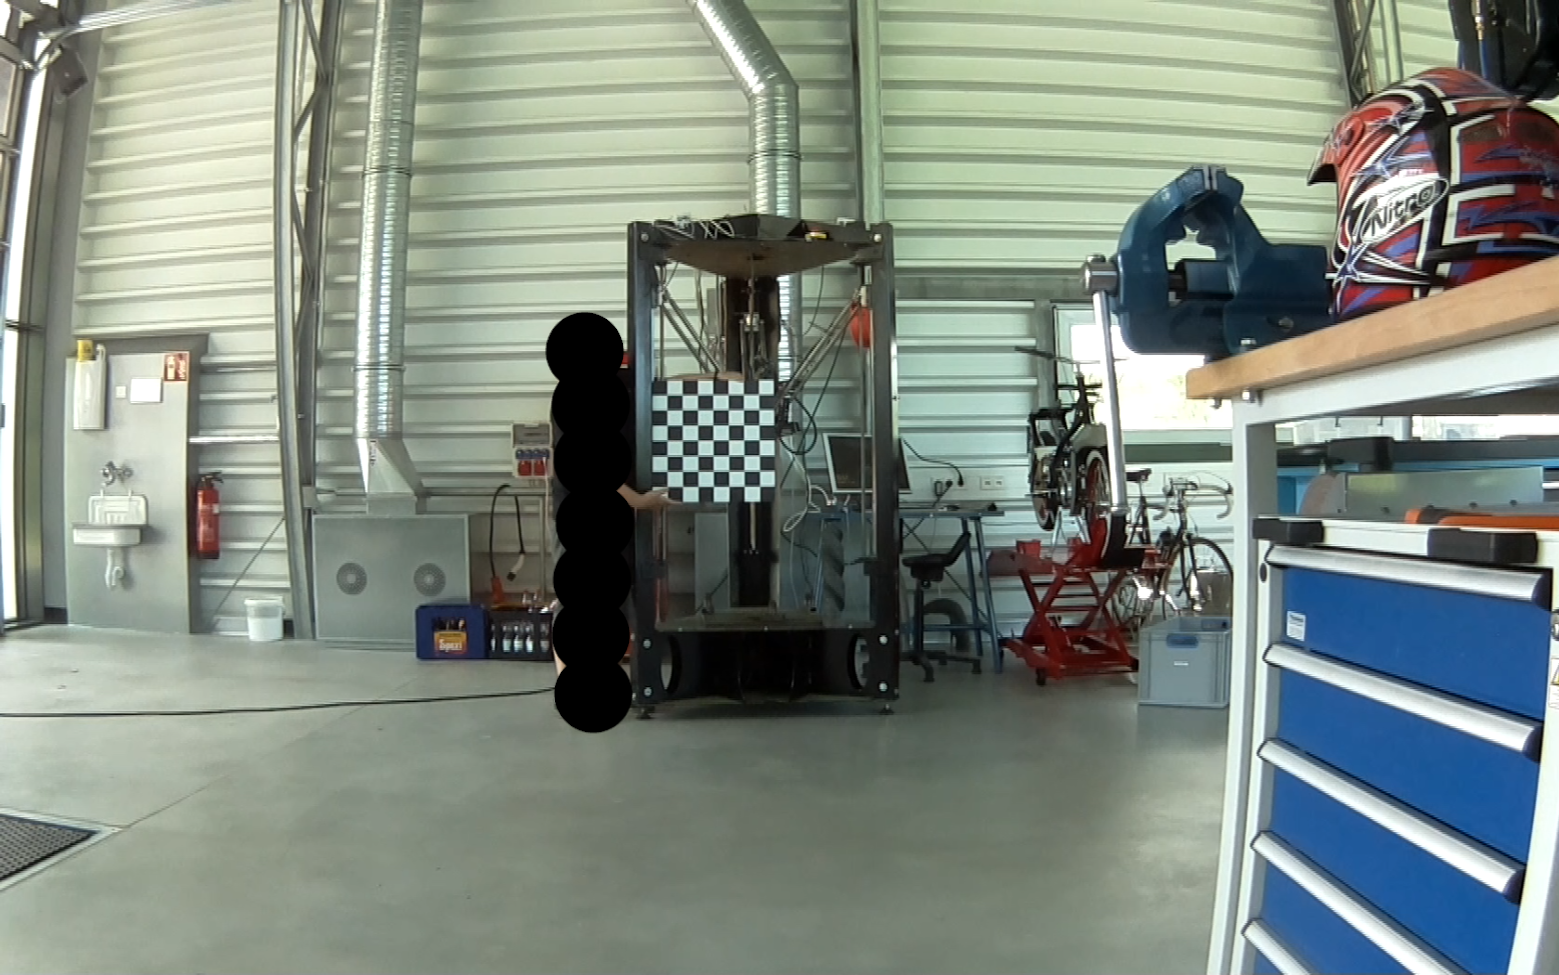
\includegraphics[width=.95\textwidth]{image/1/metal_printer.png}
        \caption{Object 3D metal printer}
        \label{fig:printer_og}
     \end{minipage}
\end{figure}

The additional goals for this project are:
\begin{itemize}[leftmargin=0.9cm]
    \item Calibrate the camera for each video separately.
    \item Provide your distance estimation  for the Schwalbe and the 3D metal printer.
    \item Provide your width and height estimation for the 3D metal printer.
\end{itemize}
    
